\section{Preliminaries}
\label{sec:preliminaries}



\subsection{Constraint Graph}
\begin{figure}[htb]
    \begin{center}
        \begin{tabular}{cc}
            \begin{minipage}{0.45\linewidth}
                \begin{center}
                    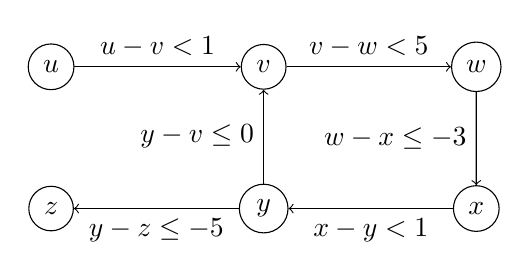
\begin{tikzpicture}[scale=0.9,state/.style={draw, circle, fill=none,text centered, text=black}]
    \node[state] (u) at (0, 2) {$u$};
    \node[state] (v) at (3, 2) {$v$};
    \node[state] (w) at (6, 2) {$w$};
    \node[state] (x) at (6, 0) {$x$};
    \node[state] (y) at (3, 0) {$y$};
    \node[state] (z) at (0, 0) {$z$};
    \draw [->] (u) -- node[anchor=south] {$ u-v < 1 $} (v);
    \draw [->] (v) -- node[anchor=south] {$ v-w < 5 $} (w);
    \draw [->] (w) -- node[anchor=east] {$ w-x \leq -3 $} (x);
    \draw [->] (x) -- node[anchor=north] {$ x-y < 1 $} (y);
    \draw [->] (y) -- node[anchor=north] {$ y-z \leq -5 $} (z);
    \draw [->] (y) -- node[anchor=east] {$ y-v \leq 0 $} (v);
\end{tikzpicture}

                \end{center}
            \end{minipage}
            &
            \begin{minipage}{0.45\linewidth}
                \begin{center}
                    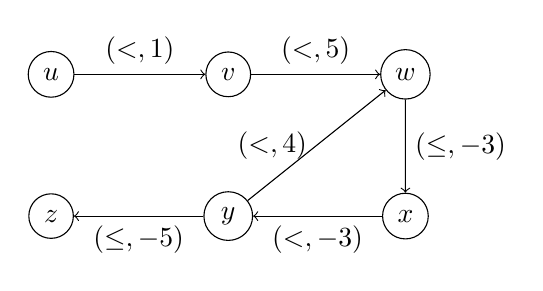
\begin{tikzpicture}[scale=0.9,state/.style={draw, circle, fill=none,text centered, text=black}]
    \node[state] (u) at (0, 2) {$u$};
    \node[state] (v) at (2.5, 2) {$v$};
    \node[state] (w) at (5, 2) {$w$};
    \node[state] (x) at (5, 0) {$x$};
    \node[state] (y) at (2.5, 0) {$y$};
    \node[state] (z) at (0, 0) {$z$};
    \draw [->] (u) -- node[anchor=south] {$ (<,1) $} (v);
    \draw [->] (v) -- node[anchor=south] {$ (<,5) $} (w);
    \draw [->] (w) -- node[anchor=west] {$ (\leq,-3) $} (x);
    \draw [->] (x) -- node[anchor=north] {$ (<,-3) $} (y);
    \draw [->] (y) -- node[anchor=north] {$ (\leq,-5) $} (z);
    \draw [->] (y) -- node[anchor=east] {$ (<,4) $} (w);
\end{tikzpicture}

                \end{center}
            \end{minipage}
        \end{tabular}
    \end{center}
    \caption{Examples of constraint graphs for
        Equation~\ref{eq:example-2} (left) and
        Equation~\ref{eq:example-3} (right).}
    \label{fig:contraints-graphs}
\end{figure}
Constraint Graph (Figure~\ref{fig:contraints-graphs})
is used by the DL constraints checker
(Figure~\ref{fig:lazy-and-incremental-approaches}).
It represents the DL constraints and allows calculate transitivity
relations between them (\eg Equation~\ref{eq:transitivity-example}).
According to~\cite{cotton2004some} this graph is defined as follows:
\begin{definition}[Constraint Graph]
    The constraint graph of a set (or conjunction) of
    DL constraints $ \Gamma $ is a graph $ \Gamma = (V,E,\xi) $
    with one vertex per numeric variable occurring in some DL
    constraint in $ \Gamma $, edges
    $ E = \{(x,y): (x - y \prec c) \in \Gamma \; for \; some \; (\prec, c) \in B \}$
    and a function $ \xi: E \mapsto B $ defined
    by $ (x,y) \mapsto \min\{(\prec, c) : (x-y \prec c) \in \Gamma\} $.
\end{definition}
Where $ \prec \in \{ <, \leq \} $,
$ B = \{ (\prec, c) \} $ is a set of bounds.
On $ B $ an order is defined as follows:
$ (\prec, c) <_B (\prec', c') $ when $ c < c' $
or when $ c = c' $ and $ \prec $ is $ < $ and $ \prec' $ is $ \leq $.
A couple of examples are given below:
\begin{equation}
    \begin{aligned}
        (\leq, -3) <_B (<, -1) \\
        (<, -1) <_B (\leq, -1) \\
    \end{aligned}
\end{equation}



\subsection{Bellman-Ford Algorithm}
Bellman-Ford algorithm~\cite[p.651]{cormen2009introduction} calculates
shortest paths from a single source vertex to all others.
It can also detect negative cycles.
In~\cite{cotton2004some} a Goldberg-Radzik~\cite{cormen2009introduction}
variant of the Bellman-Ford algorithm is used.
The algorithm is given below:
\begin{Algorithm}
    \caption{A basic SAT checking algorithm for solving SAT problem of PL.
        It takes a PL formula to be checked for satisfiability and
        returns SAT status of the formula (SAT or UNSAT)
        and, in case when the formula is SAT, a model \ie an assignment, which evaluates the formula to $ True $.}
    \label{alg:bellman-ford}
    \begin{algorithm}{procedure Scan}
        {\text{PL formula} \phi}
        model \= \varnothing \\
        (inferredAssignments, conflictingClauses) \= \CALL{Propagate}(\phi, model) \\
        conflictHasArisen \= conflictingClauses \neq \varnothing \\
        \begin{IF}{conflictHasArisen}
            \RETURN (UNSAT, \NIL)
        \end{IF} \\
        model\=model \cup inferredAssignments \\
        \begin{WHILE}{True}
            (nextVariable, value) \= \CALL{Decide}(\phi, model) \\
            allVariablesHaveAlreadyBeenAssigned \= nextVariable = \NIL \\
            \begin{IF}{allVariablesHaveAlreadyBeenAssigned}
                \RETURN (SAT, model)
            \end{IF} \\
            model \= model \cup \{ nextVariable \= value \} \\
            \begin{REPEAT} \\
                (inferredAssignments, conflictingClauses) \= \CALL{Propagate}(\phi, model) \\
                model \= model \cup inferredAssignments \\
                conflictHasArisen \= conflictingClauses \neq \varnothing \\
                \begin{IF}{conflictHasArisen}
                    (newModelWithoutConflict, \phi_a) \= \CALL{Resolve}(\phi, model, conflictingClauses) \\
                    conflictHasNotBeenResolved \= newModelWithoutConflict = \NIL \\
                    \begin{IF}{conflictHasNotBeenResolved}
                        \RETURN (UNSAT, \NIL)
                    \end{IF} \\
                    model \= newModelWithoutConflict \\
                    \phi \= \phi \land \phi_a
                \end{IF}
            \end{REPEAT} \neg conflictHasArisen
        \end{WHILE}
    \end{algorithm}
\end{Algorithm}